% \documentclass[a4paper,11pt]{article}
% \usepackage[hyperref]{beamerarticle}

\documentclass[final]{beamer}

\usepackage{kotex}
\usepackage{amsfonts,amsmath,xob-amssymb}
\usepackage{graphicx}

\usepackage{amsthm}
\newtheorem{defn}{Definition}
\newtheorem{thm}{Theorem}

\usepackage{cancel}
\usepackage{enumerate}

\mode<presentation>{
	\usetheme{Madrid}
	\usecolortheme{default}
	\usefonttheme{professionalfonts}
}

\def\b{\boldsymbol}

\mode<article>{
\usepackage{fullpage}
}
\usepackage{ulem}

\newcommand{\bb}{\mathbb}
\newcommand{\bd}{\mathbf}
\newcommand{\p}{\partial}

\newcommand{\mail}{\url{econMath.namun@gmail.com}}

\author[조남운]{\mail}
\title{Calculus of Several Variables}
\subtitle{Ch.14}

\begin{document}

\maketitle

\mode<presentation>{
\begin{frame}[t]{Table of Contents}
	\tableofcontents
\end{frame}
%--- Next Frame ---%
}

\section{Definitions and Examples} % (fold)
\label{sec:definitions_and_examples}
\begin{frame}[t]{Partial Derivative}
	Let $f:D\in\bb{R}^n\rightarrow\bb{R}$ and  $\bd{e_i}$ be a vector whose $i$ th element is 1 and others are 0.
	\[
		\bd{e_i}:= (\overbrace{0,0,\cdots,0,1}^{i},0,\cdots,0)
	\]
	\begin{defn}
		[Partial Derivative]
		\uline{Partial derivative} at $\bar{\bd{x_0}}\in D$ is \[
			\frac{\p f}{\p x_i}:= \lim_{h\rightarrow 0}\frac{f(\overline{\bd{x_0}}+h\bd{e_i})-f(\overline{\bd{x_0}})}{h}
		\]
	\end{defn}
	When $n=1$, partial derivative is equivalent to derivative of one variable function.
	\begin{block}
		{Calculation Procedure}
		\begin{itemize}
			\item Treat $x_i$ as the only variable in $f$
			\item Treat $x_{-i}$ as constant
		\end{itemize}
	\end{block}
\end{frame}
%--- Next Frame ---%
% section definitions_and_examples (end)

\section{Economic Interpretation} % (fold)
\label{sec:economic_interpretation}
\subsection{Marginal } % (fold)
\label{sub:marginal_products}
\begin{frame}[t]{Marginal Products}
	\begin{block}
		{Production Function, Marginal Product of Labor [or Capital]}
		Let $Q$ be the production function of a firm. If the firm's resources for production are $\bd{x}=(L,\bd{K})=(L,K_1,K_2,\cdots,K_N)$, \[
			MP_L:= \frac{\p Q}{\p L},\quad MP_{K_i}:=\frac{\p Q}{\p K_i}
		\]
	\end{block}
	Interpretation: Small change $\Delta K_i$ ($ceteris~paribus$) in $K_i$ can cause output change $\Delta Q$ around $(L^\ast,\bd{K}^\ast)$
	\[
		\Delta Q \approx \frac{\p Q}{\p K_i} (L^\ast,\bd{K}^\ast) \Delta K_i
	\]
	\begin{block}
		{Marginal Utility}
		Let $U(\bd{x})$ be the utility function with respect to commodity bundle $\bd{x}$. Then $\frac{\p U}{\p x_i}$ is \uline{marginal utility} of commodity $i$ at $\bd x^\ast$
	\end{block}
\end{frame}
%--- Next Frame ---%
% subsection marginal_products (end)
\subsection{Elasticity} % (fold)
\label{sub:elasticity}
\begin{frame}[t]{Elasticity}
	\begin{block}
		{Elasticity: Multi variable version} $x_i$ elasticity of $Q(\bd x)$ around $(\bd{x}^\ast,Q^\ast)$ is:\[
			\epsilon_i := \frac{\frac{\p Q}{Q^\ast}}{\frac{\p x_i}{ x_i^\ast}} = \frac{x_i^\ast}{Q^\ast}\frac{\p Q}{\p x_i}(\bd{x}^\ast)
		\]
	\end{block}
	In general, elasticity is ratio of rates of changes. When the sign of elasticity is not important, $|\epsilon|$ can be used.
\end{frame}
%--- Next Frame ---%
% subsection elasticity (end)
% section economic_interpretation (end)
\section{Geometric Interpretation} % (fold)
\label{sec:geometric_interpretation}
\begin{frame}[t]{Partial Derivative: Geometric Interpretation}
	\begin{block}
		{$f:\bb{R}^2\rightarrow \bb{R}$}
		\begin{itemize}
			\item Think of $f(\bd{x})=x_1^2 + x_2^2$.
			\item If $x_2 = \bar x_2$, $f(x_1, \bar x_2)$ is equivalent to one variable function $\tilde f(x_1) = x_1^2 + \bar x_2^2$.
			\item Graph of $\tilde f$ is intersection of the graph of $f$ with the slice $x_2=\bar x_2$.
			\item $\frac{\p f}{\p x_1}(\bar x_1, \bar x_2) = \frac{\p \tilde f}{\p x_1}(\bar x_1)$ is the slope of $\tilde f$ on $\bar x_1$, slope of the tangent line to the curve $\tilde f$ (on the plane $x_2=\bar x_2$)
		\end{itemize}
	\end{block}
\end{frame}
%--- Next Frame ---%
\begin{frame}[t]{Example}
	\begin{figure}[h]
	  \centering
	    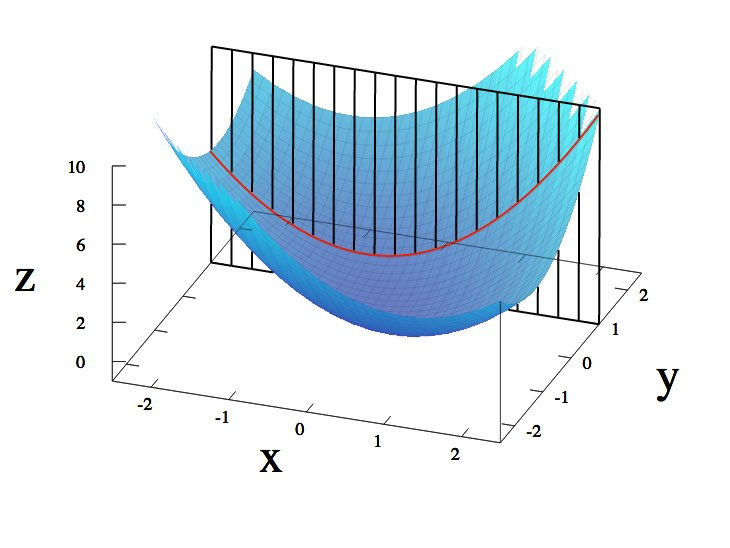
\includegraphics[width=.7\textwidth]{_img/PartialDerivative01.jpg}
		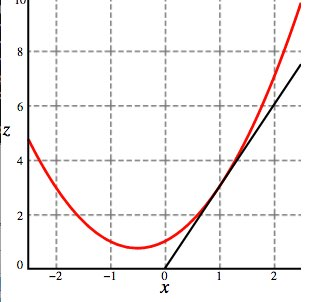
\includegraphics[width=.3\textwidth]{_img/PartialDerivative02.jpg}
	  \caption{Graph of $z = x^2 + xy + y^2$ with intersection $y=1$}
	  \label{fig:_img_partialDerivative1}
	\end{figure}
\end{frame}
%--- Next Frame ---%
% section geometric_interpretation (end)
\section{The Total Derivative} % (fold)
\label{sec:the_total_derivative}

\begin{frame}[t]{Geometrical Approach}
	\begin{block}{Finding Tangent Plane}
		Let $f:\bb{R}^2\rightarrow \bb{R}$ is differentiable. When finding a tangent plane on $(\bar x_1, \bar x_2)$, we need to get at least two independent vectors: $\left(1,0,\frac{\p f}{\p x_1}(\bar x_1, \bar x_2)\right)$ (slice $x_2=\bar x_2$), and $\left(0,1,\frac{\p f}{\p x_2}(\bar x_1, \bar x_2)\right)$ (slice $x_1=\bar x_1$)

		Then the tangent plane with two parameters $\Delta x_1, \Delta x_2$ is:\[
			(\bar {x_1}, \bar{x_2}, f(\bar {\bd x})) + \Delta x_1\left(1,0,\frac{\p f}{\p x_1}(\bar x_1, \bar x_2) \right)+\Delta x_2\left(0,1,\frac{\p f}{\p x_2}(\bar x_1, \bar x_2)\right)
		\]\[
			=\left(\bar{ x_1}+\Delta x_1 , \bar{x_2}+\Delta x_2, f(\bar {\bd x})+ \frac{\p f}{\p x_1}(\bar x_1, \bar x_2)\Delta x_1 + \frac{\p f}{\p x_2}(\bar x_1, \bar x_2)\Delta x_2 \right)
		\]
	\end{block}
	This interpretation can be extended to $n$ dimension.
\end{frame}
%--- Next Frame ---%

\begin{frame}[t]{The Total Derivative}
	\begin{block}
		{Changes in All Direction: $f:\bb{R}^n\rightarrow \bb{R}^1$}
		Let $d \bd x = (d x_1, \cdots, d x_n)$ and $f:\bb{R}^n\rightarrow\bb{R}$, differentiable. Then small change of $d\bd x$ will cause small change of $df=f(\bar{\bd x} + d \bar{\bd x}) - f(\bar{\bd x})\in\bb{R}$ and \[
			df = f(\bar{\bd x} + d \bar{\bd x}) - f(\bar{\bd x}) = \frac{\p f}{\p x_1}(\bar{\bd x})dx_1 + \cdots +\frac{\p f}{\p x_n}(\bar{\bd x})dx_n= Df_{\bd x} d\bd x
		\]
		And $Df_{\bd x}:=\begin{pmatrix}
			\frac{\p f}{\p x_1}(\bar{\bd x}) & \frac{\p f}{\p x_2}(\bar{\bd x}) &\cdots & \frac{\p f}{\p x_n}(\bar{\bd x})
		\end{pmatrix}$: (Jacobian) derivative of $f$ at $\bar{\bd x}$ or The linear approximation of $f$ at $\bar{\bd x}$, or Gradient vector $\nabla f$
	\end{block}
	Note: In this case, $Df_{\bd x}$ is a vector or $1\times n$ matrix.
\end{frame}
%--- Next Frame ---%

\begin{frame}[t]{More General Case}
	\begin{block}
		{Changes in All Direction: $\bd f:\bb{R}^n\rightarrow \bb{R}^m$}
		Let $d \bd x = (d x_1, \cdots, d x_n)$ and $\bd f:\bb{R}^n\rightarrow\bb{R}^m$, differentiable. Then small change of $d\bd x$ will cause small change of $d\bd f=\bd f(\bar{\bd x} + d \bar{\bd x}) - \bd f(\bar{\bd x})\in\bb{R}^m$ and \[
			d\bd f = \bd f(\bar{\bd x} + d \bar{\bd x}) - \bd f(\bar{\bd x}) = \frac{\p \bd f}{\p x_1}(\bar{\bd x})dx_1 + \cdots +\frac{\p \bd f}{\p x_n}(\bar{\bd x})dx_n= D\bd f_{\bd x} d\bd x
		\]
	\end{block}
	Note: In this case, $D\bd f_{\bd x}$ is $m\times n$ matrix
\end{frame}
%--- Next Frame ---%
% section the_total_derivative (end)
\section{The Chain Rule} % (fold)
\label{sec:the_chain_rule}
\begin{frame}[t]{Curve in $\bb{R}^n$}
	\begin{defn}
		[curve] A \uline{curve} in $\bb{R}^n$ is $n$-tuple of continuous one variable functions\[
			\bd x(t) = (x_1(t),\cdots,x_n(t))
		\]
		$x_i$: coordination function, $t$: parameter
	\end{defn}
	\begin{block}
		{Velocity (or Tangent) Vector}
		$\bd{x}^\prime$ is the \uline{velocity (tangent) vector} of the curve at $t$\[
			\bd{x}^\prime := \lim_{h_j\rightarrow 0}\frac{\bd{x}(t+h_j)-\bd{x}(t)}{h_j}=(x_1^\prime(t),\cdots,x_n^\prime(t))
		\]
	\end{block}
	Geometrically, The velocity (tangent) vector is a limit of secant vector
\end{frame}
%--- Next Frame ---%
\begin{frame}[t]{Regular, cusp}
	\begin{defn}
		[regular] A curve $\bd x(t)$ is regular iff $x_i^\prime(t) $ is continuous and $\bd x^\prime(t)\neq \bd{0}\quad \forall t$

		When $\bd x^\prime(\bar t) = \bd{0}$, this curve has \uline{cusp} at $\bd{x}(\bar t)$
	\end{defn}
	Geometrically, regular curve means smooth curve

	\begin{defn}
		[continuously differentiable] $f:\bb{R}^n\rightarrow\bb{R}$ is \uline{continuously differentiable} (or $C^1$) on an open set $ D\subset\bb{R}^n$ iff \[
			\forall\bd x\in D, \forall i, \quad \exists \frac{\p f}{\p x_i}(\bd x) \quad\land\quad continuous
		\]
	\end{defn}
\end{frame}
%--- Next Frame ---%

\begin{frame}[t]{Chain Rule I}
	\begin{block}
		{Chain Rule I}
		Let $g(t)=f(\bd{x}(t))$, $g:\bb{R}\rightarrow\bb{R}$, $f:\bb{R}^n\rightarrow\bb{R}$, $\bd x :\bb{R}\rightarrow\bb{R}^n$. Then, \[
			\frac{d g}{dt} = Df_{\bd x}(\bd x) \frac {d\bd x(t)}{dt} = \frac{\p f}{\p x_1}\frac{dx_1}{dt}+ \cdots +\frac{\p f}{\p x_n}\frac{dx_n}{dt}
		\]
	\end{block}
	\begin{block}
		{Chain Rule II}
		Let $g(\bd t)=f(\bd{x}(\bd t))$, $g:\bb{R}^s\rightarrow\bb{R}$, $f:\bb{R}^n\rightarrow\bb{R}$, $\bd x :\bb{R}^s\rightarrow\bb{R}^n$. Then, \[
			Dg_{\bd t} = Df_{\bd x}(\bd x) D {\bd x_{\bd t}(\bd t)}
			\]\[
				\frac{\p g}{\p t_i} = \begin{pmatrix}
					\frac{\p f}{\p x_1} & \cdots & \frac{\p f}{\p x_n}
				\end{pmatrix}\begin{pmatrix}
					\frac{\p x_1 }{\p t_1}\\
					\vdots\\
					\frac{\p x_n }{\p t_i}
				\end{pmatrix}
			\]
	\end{block}
\end{frame}
%--- Next Frame ---%
% section the_chain_rule (end)
\section{Directional Derivatives and Gradients} % (fold)
\label{sec:directional_derivatives_and_gradients}
\begin{frame}[t]{Directional Derivatives and Gradients}
	\begin{block}
		{Directional Derivative}Let $\bd x = \overline{\bd x} + t \overline{\bd v}$: line passing $\overline{\bd x}$ with direction $\overline{\bd v}$ and $g(t) = f(\overline{\bd x} + t \overline{\bd v})$. From chain rule I, \[
			\left.\frac{dg}{dt}\right\vert_{t=0} = \left.\frac{df}{dt}\right\vert_{t=0}= Df_{\bd x} (\overline{\bd x}) \cdot \frac{d\bd x}{dt} = Df_{\bd x} (\overline{\bd x})\cdot\overline{\bd v}
		\]This is the derivative of $f$ at $\overline{\bd x}$ in the direction $\overline{\bd v}$, and other notations are $\frac{\p f}{\p \bd v}(\overline{\bd x})$ and $D_{\bd v}f(\overline{\bd x})$
	\end{block}
	\begin{thm}
		[14.2] At any point $\bd x\in D$ and $\nabla f \neq 0$, $\nabla f(\bd x)$ points at $x$ into the direction in which $f$ increases most rapidly
	\end{thm}
	This theorem will be used for finding normal vector of tangent hyperplane to level set.
\end{frame}
%--- Next Frame ---%
% section directional_derivatives_and_gradients (end)
\section{Explicit Functions from $\mathbb{R}^n$ to $\mathbb{R}^m$} % (fold)
\label{sec:explicit_functions_from_mathbb_r_n_to_mathbb_r_m}
\begin{frame}[t]{Chain Rule III}
	\begin{block}
		{Chain Rule III}
		Let $\bd f(\bd x): \bb{R}^n\rightarrow \bb{R}^m$, $\bd a(t):\bb{R}\rightarrow\bb{R}^n$, and $\bd g(t) = \bd f \circ \bd a (t)$. Then, \[
			\frac{d\bd g}{dt} = Df_{\bd a}(\bd a(t))\cdot \bd a^\prime (t)
		\]
	\end{block}
	\begin{block}
		{Chain Rule IV}
		Let $\bd f(\bd x): \bb{R}^n\rightarrow \bb{R}^m$, $\bd a(\bd t ):\bb{R}^s\rightarrow\bb{R}^n$, and $\bd g(\bd t) = \bd f \circ \bd a (\bd t)$. Then, \[
			{D\bd g}_{\bd t} = {D\bd f}_{\bd a} (\bd a(\bd t))\cdot D\bd a_{\bd t}
		\]
	\end{block}
\end{frame}
%--- Next Frame ---%
% section explicit_functions_from_mathbb_r_n_to_mathbb_r_m (end)
\section{Higher-order Derivatives} % (fold)
\label{sec:higher_order_derivatives}
\begin{frame}[t]{Hessian}
	\begin{defn}
		{Hessian matrix}\[
			D^2 f_{\bd x} = D(Df)_{\bd x}:=\begin{pmatrix}
				\frac{\p^2 f}{\p x_1 \p x_1} & \frac{\p^2 f}{\p x_2\p x_1} & \cdots & \frac{\p^2 f}{\p x_n \p x_1}\\
				\frac{\p^2 f}{\p x_1 \p x_2} & \frac{\p^2 f}{\p x_2\p x_2} & \cdots & \frac{\p^2 f}{\p x_n \p x_2}\\
				\vdots & \vdots & &\vdots\\
				\frac{\p^2 f}{\p x_1 \p x_n} & \frac{\p^2 f}{\p x_2\p x_n} & \cdots & \frac{\p^2 f}{\p x_n \p x_n}\\
			\end{pmatrix}
		\]
	\end{defn}
	\begin{thm}
		[14.5:Young's theorem]
		\[
			 \frac{\p^2 f}{\p x_i\p x_j} =  \frac{\p^2 f}{\p x_j\p x_i} \quad\forall i,j
		\]
	\end{thm}
	This means hessian is symmetric.
\end{frame}
%--- Next Frame ---%
% section higher_order_derivatives (end)
\end{document}
